

\newpage
\section{Requirements}

\subsection{External Interface Requirements}
\subsubsection{Registration screen}
\begin{spacing}{1.25}
\quad This mockup is related to the registration use case. It explains the registration process.
\quad To register to the system a user should fill following fields:
\begin{itemize}
   \setlength{\itemsep}{1pt}
    \setlength{\parskip}{1pt}
  \item Name
  \item Surname
  \item Calendar visibility
  \item E-mail
  \item Password

\end{itemize}

\par After filling in all te fields a user will have to press "submit" button.
\end{spacing}
\begin{figure}[tbh]
  \begin{center}
  % Requires \usepackage{graphicx}
  \includegraphics[width=80mm]{register}
    \caption{Registration screen}\label{Fig 1:}
  \end{center}
\end{figure}
\newpage
\subsubsection{Login screen}
\quad This mockup is related to the login to the system use case. It explains the login process.
\quad Registered user can login into the system filling in "e-mail" and "password" fields.
\begin{figure}[tbh]
  \begin{center}
  % Requires \usepackage{graphicx}
  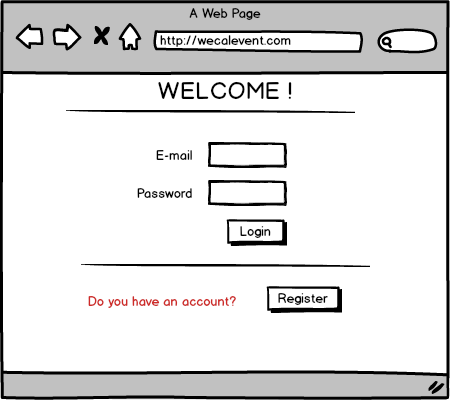
\includegraphics[width=80mm]{Login-homepage}
    \caption{Login screen}\label{Fig 2:}
  \end{center}
\end{figure}

\subsubsection{Edit profile screen}
\quad This mockup is related to the edit profile use case. It explains the edit profile process.
\quad Previously registered users are able to edit all the fields of their profile filled in during registration and calendar visibility.
\begin{figure}[tbh]
  \begin{center}
  % Requires \usepackage{graphicx}
  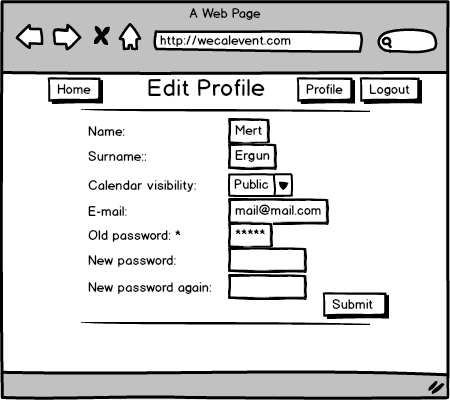
\includegraphics[width=80mm]{editprofile}
    \caption{Edit profile screen}\label{Fig 3:}
  \end{center}
\end{figure}

\subsubsection{View calendar screen}
\quad This mockup is related to the "View calendars", "Import or Export calendar", "Search event", "Search user" use case. It explains the view calendar process.
\quad Users will be able to see events they are going to participate in and events they have been invited to in a view calendar screen. On its left side users will see notification about the events. By clicking on any event related to this user she/he will see detailed information of this event and link to the list of users which have already accepted the event. By choosing anyone from this list the user will see a calendar of this person in case if it's public. The user will be able to export or import her/his calendar and search for another user or event.
\begin{figure}[tbh]
  \begin{center}
  % Requires \usepackage{graphicx}
  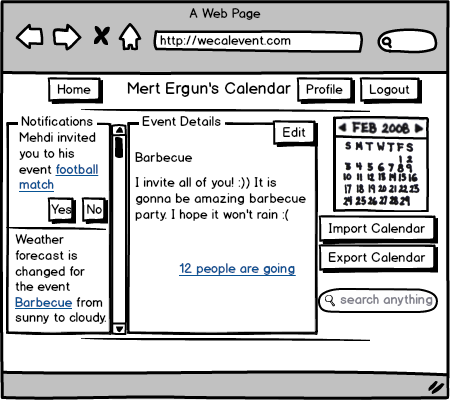
\includegraphics[width=80mm]{calendar}
    \caption{View calendar screen}\label{Fig 4:}
  \end{center}
\end{figure}
\newpage

\subsubsection{Create an event screen}
\quad This mockup is related to the "Create an event" use case. It explains the event creation process.
\quad In event creation screen (Figure 5), information about the event which will be created is
given by the user. These information are event name, event description, time, type, visibility (public, private), location, "bad" weather conditions and invited people list .
\begin{figure}[tbh]
  \begin{center}
  % Requires \usepackage{graphicx}
  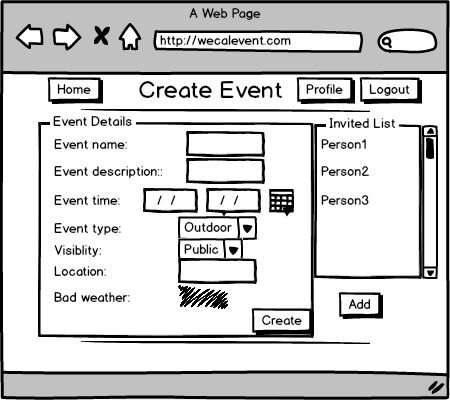
\includegraphics[width=80mm]{createevent}
    \caption{Create event screen}\label{Fig 5:}
  \end{center}
\end{figure}
\subsubsection{Edit event screen}
\quad This mockup is related to the "Edit an event" use case. It explains the event edition process.
\quad User can invite other users to the events she/he has created even after creation.
\begin{figure}[tbh]
  \begin{center}
  % Requires \usepackage{graphicx}
  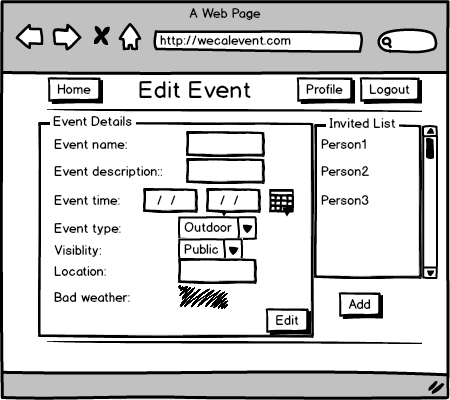
\includegraphics[width=80mm]{editevent}
  \caption{Manage event screen}\label{Fig 6:}
  \end{center}
\end{figure}

\newpage

\subsection{Functional Requirements}

\subsubsection{Registration}


\begin{tabular}{|l|l|}
  \hline
  % after \\: \hline or \cline{col1-col2} \cline{col3-col4} ...
  Name & Register to the system \\
  \hline
  Actor & User \\
  \hline
  Entry conditions & There are no entry conditions.\\
   \hline
  Flow of events &   \begin{minipage}{5in}
    \vskip 4pt
    \begin{itemize}
      \setlength{\itemsep}{1pt}
    \setlength{\parskip}{1pt}
   \item The user opens the web page.
   \item The system shows the web page to user.
   \item The user clicks on �Register� button.
   \item The system shows the form page to user.
   \item The user fills the form.
   \item The user clicks on "submit" button.

   \end{itemize}
   \vskip 4pt
 \end{minipage}\\
  \hline
  Exit conditions & \begin{minipage}{5in}
    \vskip 4pt
    \begin{itemize}
      \setlength{\itemsep}{1pt}
    \setlength{\parskip}{1pt}
   \item The system shows a success message.
   \item The system loads the home page.

   \end{itemize}
   \vskip 4pt
 \end{minipage}\\
  \hline
  Exceptions & \begin{minipage}{5in}
    \vskip 4pt
    \begin{itemize}
      \setlength{\itemsep}{1pt}
    \setlength{\parskip}{1pt}
   \item The user enters wrong inputs in some fields, then an error message is shown.
   \item The user leaves compulsory fields empty, then an error message is shown.
   \item The user refreshes the page without submit, then data is lost.

   \end{itemize}
   \vskip 4pt
 \end{minipage}\\
  \hline

\end{tabular}

\subsubsection{Login}

\begin{tabular}{|l|l|}
  \hline
  % after \\: \hline or \cline{col1-col2} \cline{col3-col4} ...
  Name & Login to the system\\
  \hline
  Actor & User \\
  \hline
  Entry conditions & User must be registered into the system .\\
   \hline
  Flow of events &   \begin{minipage}{5in}
    \vskip 4pt
    \begin{itemize}
    \setlength{\itemsep}{1pt}
    \setlength{\parskip}{1pt}
   \item The user opens the web page.
   \item The system shows the home page to user.
   \item The user enters his email and password in the input form.
   \item The user clicks on "Login" button.
   \item The system shows the calendar page.

   \end{itemize}
   \vskip 4pt
 \end{minipage}\\
  \hline
  Exit conditions & There are no exit conditions.\\
  \hline
  Exceptions & The user enters wrong email and/or password, then an error message is shown.\\
  \hline
\end{tabular}
\newpage

\subsubsection{Create an event}
\begin{tabular}{|l|l|}
  \hline
  % after \\: \hline or \cline{col1-col2} \cline{col3-col4} ...
  Name & Create an event  \\
  \hline
  Actor & User \\
  \hline
  Entry conditions & The user must be logged in.\\
   \hline
  Flow of events &   \begin{minipage}{5in}
    \vskip 4pt
    \begin{itemize}
    \setlength{\itemsep}{1pt}
    \setlength{\parskip}{1pt}
   \item The users clicks on "create an event" button.
   \item The system loads event creation page.
   \item The user fills the fields with event information.
   \item The system warns the user in case of conflict with\\ an another event and suggests to user free time.
   \item The user invites other users.
   \item The user clicks on "create" button.

   \end{itemize}
   \vskip 4pt
 \end{minipage}\\
  \hline
  Exit conditions & \begin{minipage}{5in}
    \vskip 4pt
    \begin{itemize}
    \setlength{\itemsep}{1pt}
    \setlength{\parskip}{1pt}
   \item The system shows an alert message.
   \item The calendar page is refreshed with new event.

   \end{itemize}
   \vskip 4pt
 \end{minipage}\\
  \hline
  Exceptions & \begin{minipage}{5in}
    \vskip 4pt
    \begin{itemize}
    \setlength{\itemsep}{1pt}
    \setlength{\parskip}{1pt}
   \item The user enters wrong inputs in some fields,\\ then an error message is shown.
   \item The user leaves compulsory fields empty, then an error message is shown.
   \item The user refresh the page without submit, then data is lost.

   \end{itemize}
   \vskip 4pt
 \end{minipage}\\
  \hline
\end{tabular}

\newpage

\subsubsection{Edit event}

\begin{tabular}{|l|l|}
  \hline
  % after \\: \hline or \cline{col1-col2} \cline{col3-col4} ...
  Name & Edit event \\
  \hline
  Actor & User \\
  \hline
  Entry conditions & \begin{minipage}{5in}
    \vskip 4pt
    \begin{itemize}
    \setlength{\itemsep}{1pt}
    \setlength{\parskip}{1pt}
   \item The user must be logged in.
   \item The event must be created.


   \end{itemize}
   \vskip 4pt
 \end{minipage}\\
   \hline
  Flow of events &   \begin{minipage}{5in}
    \vskip 4pt
    \begin{itemize}
    \setlength{\itemsep}{1pt}
    \setlength{\parskip}{1pt}
   \item The event creator clicks on an event.
   \item The system loads event creation page with existing\\ information.
   \item The event creator updates the event information.
   \item The system warns the user in case of conflict with\\ an another event and suggests to user free time.
   \item The user clicks on "Edit" button.

   \end{itemize}
   \vskip 4pt
 \end{minipage}\\
  \hline
  Exit conditions & \begin{minipage}{5in}
    \vskip 4pt
    \begin{itemize}
    \setlength{\itemsep}{1pt}
    \setlength{\parskip}{1pt}
   \item The system shows an alert message.
   \item The calendar page is refreshed with new event.

   \end{itemize}
   \vskip 4pt
 \end{minipage}\\
  \hline
  Exceptions & \begin{minipage}{5in}
    \vskip 4pt
    \begin{itemize}
    \setlength{\itemsep}{1pt}
    \setlength{\parskip}{1pt}
   \item The user enters wrong inputs in some fields,\\ then an error message is shown.
   \item The user leaves compulsory fields empty,\\ then an error message is shown.
   \item The user refreshes the page without submit,\\ then data is lost.

   \end{itemize}
   \vskip 4pt
 \end{minipage}\\
  \hline
\end{tabular}

\newpage

\subsubsection{Delete an event}

\begin{tabular}{|l|l|}
  \hline
  % after \\: \hline or \cline{col1-col2} \cline{col3-col4} ...
  Name & Delete an event  \\
  \hline
  Actor & User \\
  \hline
  Entry conditions & \begin{minipage}{5in}
    \vskip 4pt
    \begin{itemize}
    \setlength{\itemsep}{1pt}
    \setlength{\parskip}{1pt}
   \item The user must be logged in.
   \item The event must be created.

   \end{itemize}
   \vskip 4pt
 \end{minipage}\\
   \hline
  Flow of events &   \begin{minipage}{5in}
    \vskip 4pt
    \begin{itemize}
    \setlength{\itemsep}{1pt}
    \setlength{\parskip}{1pt}
   \item The event creator clicks on an event.
   \item The system loads event creation page with existing information.
   \item The event creator clicks on �Delete� button.
   \item The system shows a dialog box.
   \item The user clicks on "yes" button.

   \end{itemize}
   \vskip 4pt
 \end{minipage}\\
  \hline
  Exit conditions & \begin{minipage}{5in}
    \vskip 4pt
    \begin{itemize}
    \setlength{\itemsep}{1pt}
    \setlength{\parskip}{1pt}
   \item The system shows an alert message.
   \item The calendar page is refreshed without the event.

   \end{itemize}
   \vskip 4pt
 \end{minipage}\\
  \hline
  Exceptions & \begin{minipage}{5in}
    \vskip 4pt
    \begin{itemize}
    \setlength{\itemsep}{1pt}
    \setlength{\parskip}{1pt}
   \item The user clicks on "NO" button.

   \end{itemize}
   \vskip 4pt
 \end{minipage}\\
  \hline
\end{tabular}


\subsubsection{Invite users}

\begin{tabular}{|l|l|}
  \hline
  % after \\: \hline or \cline{col1-col2} \cline{col3-col4} ...
  Name & Invite users \\
  \hline
  Actor & User \\
  \hline
  Entry conditions &   \begin{minipage}{5in}
    \vskip 4pt
    \begin{itemize}
    \setlength{\itemsep}{1pt}
    \setlength{\parskip}{1pt}
   \item The user must be logged in.
   \item The event must be created.
   \item The user must be the event owner.

   \end{itemize}
   \vskip 4pt
 \end{minipage}\\
   \hline
  Flow of events &   \begin{minipage}{5in}
    \vskip 4pt
    \begin{itemize}
    \setlength{\itemsep}{1pt}
    \setlength{\parskip}{1pt}
   \item The user selects one of his events.
   \item The user clicks on "invite people" button.
   \item The user selects users to invite from the list.

   \end{itemize}
   \vskip 4pt
 \end{minipage}\\
  \hline
  Exit conditions & There are no exit conditions \\
  \hline
  Exceptions & There are no exceptions. \\
  \hline
\end{tabular}



\subsubsection{Answer event invitation}

\begin{tabular}{|l|l|}
  \hline
  % after \\: \hline or \cline{col1-col2} \cline{col3-col4} ...
  Name & Answer event invitation \\
  \hline
  Actor & User \\
  \hline
  Entry conditions &   \begin{minipage}{5in}
    \vskip 4pt
    \begin{itemize}
    \setlength{\itemsep}{1pt}
    \setlength{\parskip}{1pt}
   \item The user must be logged in.
   \item The event must be created.
   \item The user must be invited.

   \end{itemize}
   \vskip 4pt
 \end{minipage}\\
   \hline
  Flow of events &  The user accepts/declines to participate in event(s)\\
  \hline
  Exit conditions & There are no exit conditions \\
  \hline
  Exceptions & There are no exceptions. \\
  \hline
\end{tabular}

\subsubsection{Search user}

\begin{tabular}{|l|l|}
  \hline
  % after \\: \hline or \cline{col1-col2} \cline{col3-col4} ...
  Name & Search user \\
  \hline
  Actor & User \\
  \hline
  Entry conditions &  The user must be logged in.
   \\
   \hline
  Flow of events &  The user inputs the name to search for.\\
  \hline
  Exit conditions & User found. \\
  \hline
  Exceptions & No user found with that name. \\
  \hline
\end{tabular}


\subsubsection{Search event}

\begin{tabular}{|l|l|}
  \hline
  % after \\: \hline or \cline{col1-col2} \cline{col3-col4} ...
  Name & Search event \\
  \hline
  Actor & User \\
  \hline
  Entry conditions &  The user must be logged in.
\\
   \hline
  Flow of events &   The user input the event to search for.\\
  \hline
  Exit conditions & Event found. \\
  \hline
  Exceptions & No event found with that name. \\
  \hline
\end{tabular}

\subsubsection{Edit profile}

\begin{tabular}{|l|l|}
  \hline
  % after \\: \hline or \cline{col1-col2} \cline{col3-col4} ...
  Name & Edit profile \\
  \hline
  Actor & User \\
  \hline
  Entry conditions & The user must be logged in.\\
   \hline
  Flow of events &   \begin{minipage}{5in}
    \vskip 4pt
    \begin{itemize}
    \setlength{\itemsep}{1pt}
    \setlength{\parskip}{1pt}
   \item The event creator clicks on "Edit profile".
   \item The system loads personal information page with existing information.
   \item The user updates his information.
   \item The user clicks on "submit" button.
   \item The system shows the alert message.
   \item The user clicks on "yes" button.

   \end{itemize}
   \vskip 4pt
 \end{minipage}\\
  \hline
  Exit conditions & \begin{minipage}{5in}
    \vskip 4pt
    \begin{itemize}
    \setlength{\itemsep}{1pt}
    \setlength{\parskip}{1pt}
   \item The system shows an alert message.
   \item The profile page is refreshed with new personal information.

   \end{itemize}
   \vskip 4pt
 \end{minipage}\\
  \hline
  Exceptions & \begin{minipage}{5in}
    \vskip 4pt
    \begin{itemize}
    \setlength{\itemsep}{1pt}
    \setlength{\parskip}{1pt}
   \item The user enters wrong inputs in some fields, then an error message is shown.
   \item The user leaves compulsory fields empty, then an error message is shown.
   \item The user refresh the page without submit, then data is lost.

   \end{itemize}
   \vskip 4pt
 \end{minipage}\\
  \hline
\end{tabular}



\subsubsection{View Calendars}

\begin{tabular}{|l|l|}
  \hline
  % after \\: \hline or \cline{col1-col2} \cline{col3-col4} ...
  Name & View Calendars \\
  \hline
  Actor & User \\
  \hline
  Entry conditions & The user must be logged in. \\
   \hline
  Flow of events &   \begin{minipage}{5in}
    \vskip 4pt
    \begin{itemize}
    \setlength{\itemsep}{1pt}
    \setlength{\parskip}{1pt}
   \item The user selects another user.
   \item The system shows the calendar of that user.

   \end{itemize}
   \vskip 4pt
 \end{minipage}\\
  \hline
  Exit conditions & There are no exit conditions \\
  \hline
  Exceptions & The calendar is private.\\
  \hline
\end{tabular}


\subsubsection{Manage Calendar Visibility}

\begin{tabular}{|l|l|}
  \hline
  % after \\: \hline or \cline{col1-col2} \cline{col3-col4} ...
  Name & Manage Calendar Visibility \\
  \hline
  Actor & User \\
  \hline
  Entry conditions & The user must be logged in. \\
   \hline
  Flow of events &   \begin{minipage}{5in}
    \vskip 4pt
    \begin{itemize}
    \setlength{\itemsep}{1pt}
    \setlength{\parskip}{1pt}
   \item The user clicks on "edit profile" button.
   \item The user chooses to put his calendar public/private.

   \end{itemize}
   \vskip 4pt
 \end{minipage}\\
  \hline
  Exit conditions & There are no exit conditions \\
  \hline
  Exceptions & There are no exceptions.\\
  \hline
\end{tabular}

\subsubsection{Import or Export Calendar}

\begin{tabular}{|l|l|}
  \hline
  % after \\: \hline or \cline{col1-col2} \cline{col3-col4} ...
  Name & Import or Export Calendar \\
  \hline
  Actor & User \\
  \hline
  Entry conditions & The user must be logged in.\\
   \hline
  Flow of events &   \begin{minipage}{5in}
    \vskip 4pt
    \begin{itemize}
    \setlength{\itemsep}{1pt}
    \setlength{\parskip}{1pt}
   \item The user click on "import calendar" or "export calendar" buttons.
   \item If the user wants to export his calendar, the user clicks the export button. Otherwise, the user provides a valid document to import events to his calendar and the system saves the provided calendar..
   

   \end{itemize}
   \vskip 4pt
 \end{minipage}\\
  \hline
  Exit conditions & There are no exit conditions \\
  \hline
  Exceptions & If the calendar is not in the requested format, the system gives an error. \\
  \hline
\end{tabular}

\newpage

\subsubsection{Notify Users}
\begin{tabular}{|l|l|}
  \hline
  % after \\: \hline or \cline{col1-col2} \cline{col3-col4} ...
  Name & Notify Users \\
  \hline
  Actor & System \\
  \hline
  Entry conditions & \begin{minipage}{5in}
    \vskip 4pt
    \begin{itemize}
    \setlength{\itemsep}{1pt}
    \setlength{\parskip}{1pt}
   \item The user must be logged in. 
   \item The user must be owner of event.
   \item The user must be participant in that event.
   
   \end{itemize}
   \vskip 4pt
 \end{minipage}. \\
   \hline
  Flow of events &   \begin{minipage}{5in}
    \vskip 4pt
    \begin{itemize}
    \setlength{\itemsep}{1pt}
    \setlength{\parskip}{1pt}
   \item There are three conditions at which the user is notified\\ via e-mail and a notification in the application when they log in.
   \begin{itemize}
     \item 	The weather forecast will be controlled every 12 hours. In case of\\ a forecast change for an event, every user that participates in\\ the particular event will be notified.
     \item 	The system checks exactly 3 days before the event how is the weather\\ on the event time. If there is a bad weather condition, the\\ system suggests the closest possible day with\\ a good weather condition to the owner of the event.
     \item 	The system checks exactly 1 day before the event\ how is the weather\\ on the event time. If there is a bad weather condition, the \\ system notifies every user that participates in that event.
   \end{itemize}

   \end{itemize}
   \vskip 4pt
 \end{minipage}\\
  \hline
  Exit conditions & There are no exit conditions \\
  \hline
  Exceptions & There are no exceptions.\\
  \hline
\end{tabular}

\newpage

\subsection{Sequence diagrams}
\begin{figure}[tbh]
  \begin{center}
  % Requires \usepackage{graphicx}
  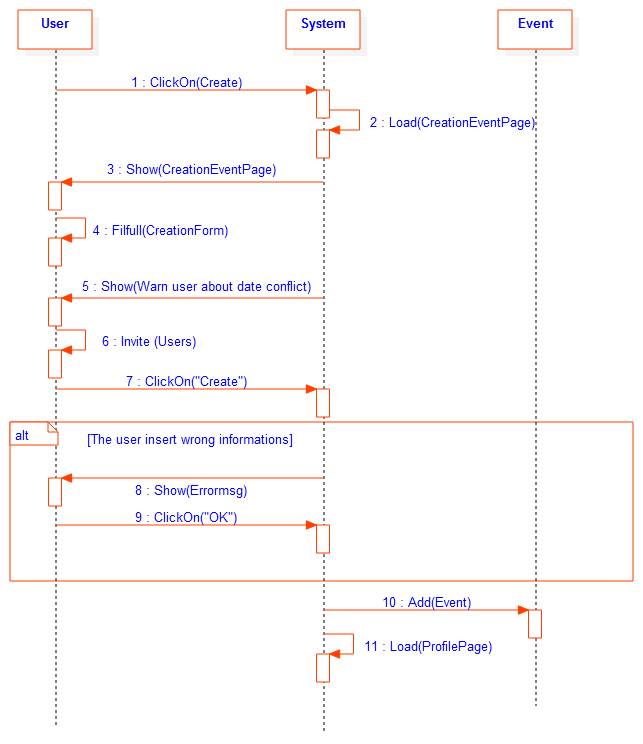
\includegraphics[width=150mm]{Create}
    \caption{Create}\label{Fig 7:}
  \end{center}
\end{figure}

\newpage

\begin{figure}[tbh]
  \begin{center}
  % Requires \usepackage{graphicx}
  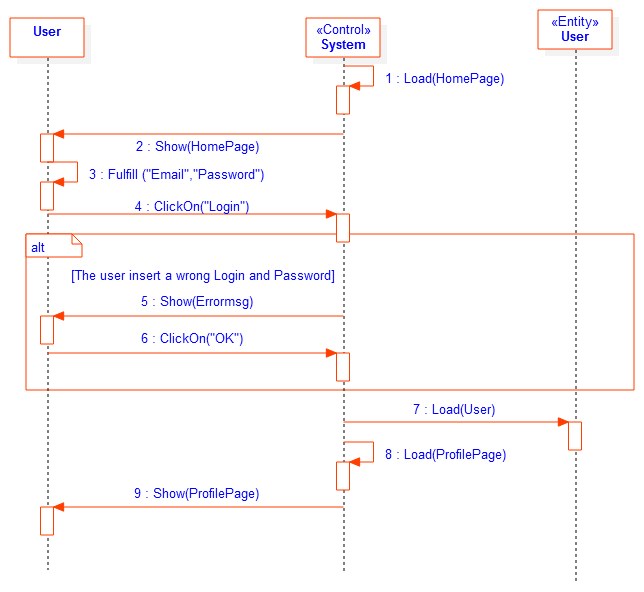
\includegraphics[width=160mm]{Login}
    \caption{Login}\label{Fig 8:}
  \end{center}
\end{figure}

\newpage

\begin{figure}[tbh]
  \begin{center}
  % Requires \usepackage{graphicx}
  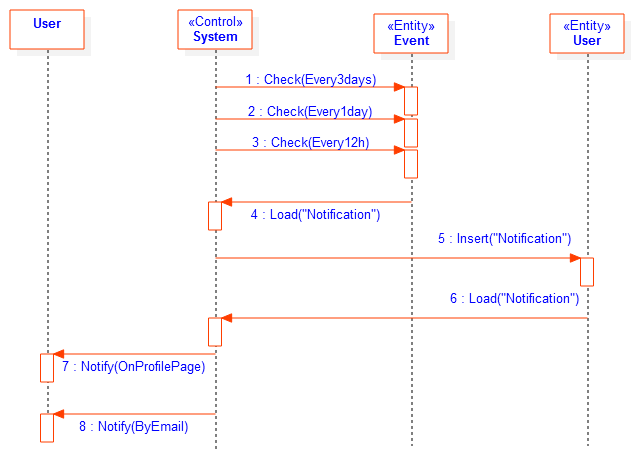
\includegraphics[width=160mm]{Notify}
    \caption{Notify}\label{Fig 9:}
  \end{center}
\end{figure}

\newpage

\begin{figure}[tbh]
  \begin{center}
  % Requires \usepackage{graphicx}
  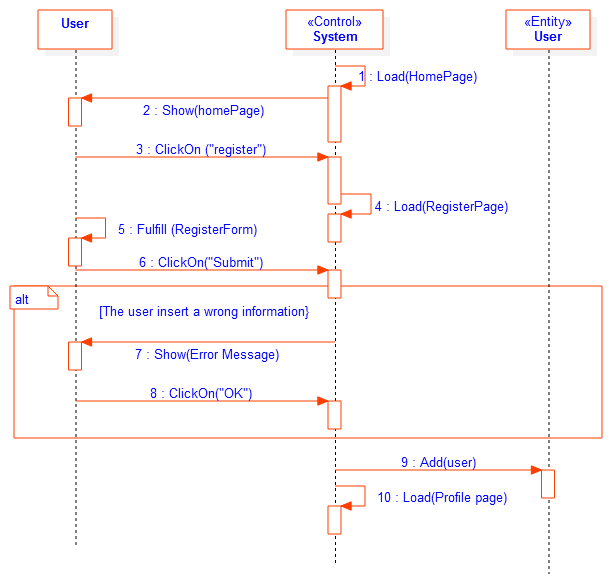
\includegraphics[width=150mm]{Register(1)}
    \caption{Register}\label{Fig 10:}
  \end{center}
\end{figure}

\newpage

\subsection{StateChart diagrams}

\begin{figure}[tbh]
  \begin{center}
  % Requires \usepackage{graphicx}
  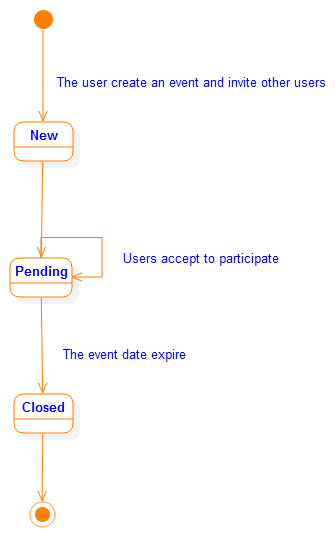
\includegraphics[width=100mm]{CreateEventd}
    \caption{Create Event}\label{Fig 11:}
  \end{center}
\end{figure}
\newpage
\begin{figure}[tbh]
  \begin{center}
  % Requires \usepackage{graphicx}
  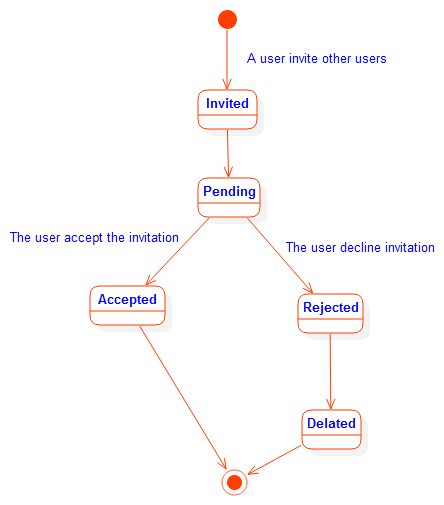
\includegraphics[width=100mm]{Inviteuserd}
    \caption{Invite User}\label{Fig 12:}
  \end{center}
\end{figure}

\newpage

\subsection{Non-functional Requirements}

\subsubsection{Reliability}
\quad The system should be able to behave consistently in a user-acceptable
manner when operating within the environment for which the system
was intended.
\subsubsection{Availability}
\quad The system should be able to deliver services when requested.
\subsubsection{Security}
\quad The system should be able to protect itself against accidental or deliberate intrusion.

\subsubsection{Maintainability}
\quad Maintainability is the parameter concerned with how the system in use can be restored after a failure. The system should periodically have back ups in order not to loose any information.

\subsubsection{Portability}
The application should easily be transferred from one computer environment to another.
